\documentclass[12pt,t]{beamer}
\usepackage{amsmath, graphicx, kbordermatrix}
\setbeameroption{hide notes}
\setbeamertemplate{note page}[plain]

% page number
\setbeamertemplate{footline}{%
    \raisebox{5pt}{\makebox[\paperwidth]{\hfill\makebox[20pt]{\color{gray}
          \scriptsize\insertframenumber}}}\hspace*{5pt}}

% add a bit of space at the top of the notes page
\addtobeamertemplate{note page}{\setlength{\parskip}{12pt}}


% a few macros
\newcommand{\subt}[1]{{\footnotesize \color{subtitle} {#1}}}

% title info
\title{Logistic Regression}
\subtitle{With an intro to sigmoid, softmax, and cross-entropy}
\author{\href{http://richcorrado.github.io}{Richard Corrado}}
\institute{Fat Cat Machine Learning}
\date{\href{https://github.com/richcorrado}{\tt \scriptsize github.com/richcorrado}}

\begin{document}

% title slide
{
	\setbeamertemplate{footline}{} % no page number here
	\frame{
		\titlepage
} } 
	


\begin{frame}{Goals}

\begin{itemize}
\item Apply neural networks to study the MNIST digit classification problem.
\item Use TensorFlow to accomplish this: requires low-level definitions of the models we will use.
\item NNs use linear models to link layers and to output.
\item Need to understand how to implement multiclass classification via linear models at a fairly low-level.
\item Understand how to map linear output to class labels: sigmoid and softmax functions
\item Understand appropriate cost function: cross-entropy
\end{itemize}


\end{frame}

\begin{frame}{Ordinary Linear Regression}

Design or Feature Matrix:
\vspace{-4mm}
$$ \mathbf{X} = \bordermatrix{ & \leftarrow & \text{feature} & \text{index} & \rightarrow \cr
		~~~\uparrow &  & &  & \cr
		\text{example} &  & & &  \cr
		\text{index} &  & & &\cr
 		~~~\downarrow &  & & &\cr
 		}$$

Response (Vector):
\vspace{-8mm}
$$ \mathbf{y} = \bordermatrix{ & ~~ &  \cr
		~~~\uparrow &    & \cr
		\text{example} &  &  \cr
		\text{index} &   &\cr
 		~~~\downarrow &   &\cr
 		}$$
We assume that $\mathbf{y} $ takes continuous values.
\end{frame}

\begin{frame}{}

Linear Parameters:
\vspace{-8mm}
$$ \text{weights}:~~~\mathbf{W} = \bordermatrix{ & ~~ &  \cr
		~~~\uparrow &    & \cr
		\text{feature} &  &  \cr
		\text{index} &   &\cr
 		~~~\downarrow &   &\cr
 		}$$

$$ \text{bias}:~~~\mathbf{b} =  \bordermatrix{ &  &  \cr
		~~~\uparrow &  b  & \cr
		\text{example} &  \vdots &  \cr
		\text{index} &  \vdots  &\cr
 		~~~\downarrow & b  &\cr
 		}$$

Then the output of a linear model
$$ \hat{\mathbf{y}}(\mathbf{X, W}, b) = \mathbf{X W} + \mathbf{b}$$
is a vector of dimension (\# of examples).
\end{frame}

\begin{frame}{Maximum Likelihood Estimate}
If $\mathbf{y}$ is a continuous response, it makes sense to assume that the errors between the true and predicted values
$$ \mathbf{\epsilon} =\mathbf{ y} - \hat{\mathbf{y}} $$
are normally distributed, then conditional probability of reproducing $\mathbf{y}$ from the model is
$$ p(\mathbf{ y} | \mathbf{ X} ) = \mathcal{N}(\mathbf{ y}; \hat{\mathbf{ y}}, \sigma^2)= \prod_i  \mathcal{N}( y_i; \hat{ y_i}, \sigma^2),$$
$$  \mathcal{N}(\mathbf{ y}; \hat{\mathbf{ y}}, \sigma^2) 
	= \frac{1}{(2\pi \sigma^2)^{n/2}} \exp \left( - \frac{1}{2\sigma^2} |\mathbf{ y}- \hat{\mathbf{ y}} |^2 \right).$$
We want to maximize the probability of obtaining predictions that have a small error compared to the true values.

\end{frame}

\begin{frame}{}
View $\mathbf{X}$ as fixed, then  $ p(\mathbf{ y} | \mathbf{ X} ) = L(\mathbf{W}, b|\mathbf{X},\mathbf{ y} )$ is the likelihood function for the parameters $\rightarrow$ find $\mathbf{W, b}$ that maximize.

\bigskip
The natural logarithm is monotonically increasing,  so equivalently maximize (log of product = sum of logs)
$$ \ln L(\mathbf{W}, b|\mathbf{X},\mathbf{ y} ) = - \frac{1}{2\sigma^2} |\mathbf{ y}- \hat{\mathbf{ y}} |^2 - \ln \sqrt{2\pi \sigma^2},$$
or {\bf minimize} the {\bf cost function}:
$$ J(\mathbf{W}, b) = |\mathbf{ y}- \hat{\mathbf{ y}} |^2,$$
by choosing appropriate parameters $\mathbf{W, b}$.  We recognize $J$ as the residual sum of squares.

\end{frame}

\begin{frame}{Gradient Descent}
Cost function is minimized when
$$ \nabla_\mathbf{W}J(\mathbf{W}, b)  =  \nabla_b J(\mathbf{W}, b) =0.$$
Since 
$$ J(\mathbf{W}, b) =  (\mathbf{X W} + \mathbf{b} -  \mathbf{y})(\mathbf{X W} + \mathbf{b} -  \mathbf{y})^T,$$
$$ \nabla_\mathbf{W}J(\mathbf{W}, b)  =  2 (\mathbf{X W} + \mathbf{b} -  \mathbf{y})^T \mathbf{X}.$$
This is a vector of dimension( \# of features).

\end{frame}

\begin{frame}{}
Consider the shift
$$ \mathbf{W}' = \mathbf{W} - \epsilon  \mathbf{V}, ~~~ \mathbf{V} = (\mathbf{X W} + \mathbf{b} -  \mathbf{y})^T \mathbf{X},$$
where $\epsilon > 0$. Then we can show that
$$ J(\mathbf{W}', b) = J(\mathbf{W}, b)  
- 2 \epsilon | \mathbf{V}|^2
%   (\mathbf{X W} + \mathbf{b} -  \mathbf{y})^T \mathbf{X} (\mathbf{X W} + \mathbf{b} -  \mathbf{y})^T \mathbf{X }
+ \mathcal{O}(\epsilon^2).$$
Therefore, for small enough $\epsilon$,  we have $ J(\mathbf{W}', b) < J(\mathbf{W}, b) $, {\it i.e.}, we have reduced the cost function by this change of parameters.

\bigskip
{\bf Gradient descent algorithm}: 

\bigskip
{\bf while} $J(\mathbf{W}, b) > \delta$: ~~~\# tolerance parameter $\delta >0$
 $~~~~ \mathbf{W} = \mathbf{W} - \epsilon (\mathbf{X W} + \mathbf{b} -  \mathbf{y})^T \mathbf{X}$

\bigskip
$\epsilon$ is usually called the {\bf learning rate}.
\end{frame}

\begin{frame}{}
For the linear model, the cost function is convex:

\centerline{
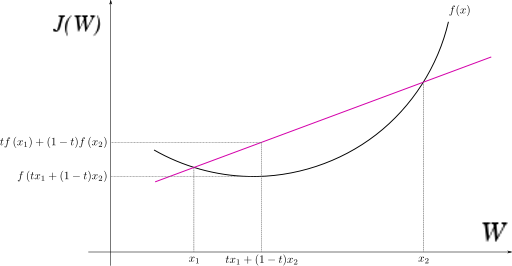
\includegraphics[height=0.5\textheight]{ConvexFunction.png}
}

This implies that gradient descent will converge in a neighborhood of the true global minimum for appropriately small $\epsilon, \delta$.

\bigskip

For general optimization problems, gradient descent is not guaranteed to converge, or if it does, it might find a local minimum.
\end{frame}

\begin{frame}{Binary Response}
If the response  $\mathbf{y}$ is not continuous, but discrete, the previous analysis based on Normal distribution of errors is invalid.  Suppose that we have a binary response, taking values $y  =0,1$.   Now we need to specify $p(y=1|\mathbf{X})$, since
$$ p(y=1|\mathbf{X}) + p(y=0|\mathbf{X}) =1.$$

{\bf Problem}: find $\phi(z)$ so that:
$$ p(y=1|\mathbf{X}) = \phi(z), ~~ z = \mathbf{X W} +b,$$
subject to $ 0 < \phi(z)< 1$, while $-\infty < z < \infty$.


\end{frame}

\begin{frame}{}

Have:
$$-\infty < z < \infty,$$
$$ 0 < \phi(z)< 1.$$ 
Note that 
$$ -\infty <\ln \phi(z)< 0,$$ 
$$ 0 < - \ln(1-\phi(z))< \infty,$$
and so 
$$ -\infty <\ln \phi(z) - \ln(1-\phi(z))< \infty.$$ 
Then
$$ \ln\left(\frac{ \phi(z)}{1-\phi(z)} \right)= z,$$
$$ \phi(z) = \frac{e^z}{1 + e^z} $$
is a reasonable choice.  This is the {\bf sigmoid function}.

\end{frame}

\begin{frame}{Sigmoid or Logistic Function}
$$ \phi(z) = \frac{e^z}{1 + e^z} $$
\centerline{
\includegraphics[height=0.4\textheight]{Logistic-curve.png}
}


\begin{itemize}
\item Rapidly changing near decision boundary $z = 0 $.
\item Well-behaved derivatives for gradient descent.
\end{itemize}

\end{frame}

\begin{frame}{Bernoulli Distribution}
$$ p(y=1|\mathbf{X}) =  \phi(z)  = \frac{e^z}{1 + e^z},$$
$$ p(y=0|\mathbf{X}) = 1- \phi(z)  = \frac{1}{1 + e^z},$$
$$ p(y|\mathbf{X}) = \phi(z)^y (1- \phi(z) )^{1-y} = \frac{e^{yz}}{\sum_{y' =0}^1 e^{y'z}}.$$

\begin{itemize}
\item $q_{\hat{y}=1}  = \phi(z)$ is model probability to find $\hat{y}=1$.
\item $q_{\hat{y}=0}  =1-\phi(z)$ is model probability to  find $\hat{y}=0$.
\item $p_{y=1}  =y$ is true probability that $y=1$.
\item $p_{y=0}  =1-y$ is is true probability that $y=0$.
\end{itemize}
\end{frame}

\begin{frame}{Cost Function}
As before, applying the maximum likelihood principal to $p(y|\mathbf{X}) $ leads to minimizing the cost function
\begin{equation*}\begin{split}
J (\text{one example}) =&  - \ln p(y|\mathbf{X}) \\
= &- y \ln \phi(z) - (1-y) \ln (1- \phi(z)) \\
= & - p_{y=1} \ln q_{y=1}  - p_{y=0} \ln q_{y=0} \\
= & - \sum_{y=0}^1 p(y) \ln q(\hat{y}) \\
= & \mathbb{E}_p \left[ - \ln q\right].
\end{split}\end{equation*} 
This expectation value is called the {\bf cross-entropy} between the  model distribution $q(\hat{y})$ and the true distribution $p(y)$.

\end{frame}

\begin{frame}{Multiclass Classification}
Suppose now we have $C$ classes, which is equivalent to $y = 0, 1, \ldots, C-1$.

\bigskip
{\bf One vs. All Scheme}: \\
For each class $c$, have a binary classification between $y=c$ and $y \neq c$.

\bigskip
{\bf One Hot Encoding}:\\
Replace class labels with vector representation:
\begin{equation*}\begin{split} 
0 \rightarrow  &(1, 0, \ldots, 0) \\
1 \rightarrow & (0, 1, \ldots, 0) \\
&~~~~ \vdots \\
C-1  \rightarrow &(0, 0, \ldots, 0,1 ).
\end{split}\end{equation*} 

\end{frame}

\begin{frame}{Scikit-Learn LabelBinarizer}

\centerline{
\includegraphics[height=0.7\textheight]{labelbinarizer.png}
}


\end{frame}

\begin{frame}{Argmax Function}

Note: Class label maps to index of nonzero element of class vector. 

\centerline{
\includegraphics[height=0.4\textheight]{numpyargmax.png}
}

Map back to class labels:

\centerline{
\includegraphics[height=0.3\textheight]{numpyargmax2.png}
}

\end{frame}

\begin{frame}{New Linear Model}

\vspace{-8mm}
$$ \text{weights}:~~~\mathbf{W} = \bordermatrix{ & \leftarrow & \text{class} & \text{index} & \rightarrow  \cr
		~~~\uparrow &    & &    &\cr
		\text{feature} &  & &    & \cr
		\text{index} &   &&    &\cr
 		~~~\downarrow &   &&    &\cr
 		}$$

$$ \text{bias}:~~~\mathbf{b} =  \bordermatrix{ & \leftarrow & \text{class} & \text{index} & \rightarrow  \cr
		~~~\uparrow &  b  &\cdots& \cdots   & b\cr
		\text{example} &  \vdots &  &    &\vdots\cr
		\text{index} &  \vdots  &&    &\vdots\cr
 		~~~\downarrow & b  &\cdots&  \cdots &b\cr
 		}$$

$$ \mathbf{z}(\mathbf{X, W}, b) = \mathbf{X W} + \mathbf{b}$$
is an array of dimension (\# of examples) $\times$ ( \# of classes).
\end{frame}

\begin{frame}{Class Probabilities}

Convert $\mathbf{z}$ to class probabilities with {\bf softmax function}:
$$ \text{softmax}(\mathbf{z})_c = \frac{\exp(z_c)}{\sum_a \exp(z_a)}, $$
$$ \text{softmax}(\mathbf{z}) = \frac{1}{\sum_a e^{z_a}} \Bigl(e^{z_0}, e^{z_1}, \ldots, e^{z_{C-1}}\Bigr). $$

\begin{itemize}
\item Each element is in $[0,1]$.
\item Sum over  elements $=1$
\item Maximum value of $\exp(z_c)$ determines the most probable class $\rightarrow$ can find it with \texttt{numpy.argmax}.
\end{itemize}
\end{frame}

\begin{frame}{Cost Function}
the new cost function is sometimes called the {\bf softmax cross-entropy}
$$
J (\text{example}~i) = \sum_{i=c}^C y_{ic}   \ln \text{softmax}(z)_{ic},
$$
\begin{itemize}
\item $y_{ic} = 1$ iff example $i$ is in class $c$. \\
\item $\text{softmax}(z)_{ic}$ is the model probability that  the example $i$ is in class $c$.
\end{itemize} 
\end{frame}

\begin{frame}{Scikit-Learn LogisticRegression}

\centerline{
\includegraphics[height=0.8\textheight]{Log_proba.png}
}
\end{frame}

\begin{frame}{Review}
\begin{itemize}
\item We've learned the necessary ingredients  to use the output of a neural network to do multiclass classification at a low-level.
\item This will be useful when we apply TensorFlow to build neural networks for, e.g., the MNIST digit problem.
\item We've learned the role of the sigmoid, softmax and cross-entropy cost function in multiclass classification.
\item We've seen some tools from numpy and scikit-learn that help us with one hot encoding and one vs. all classification schemes.
\end{itemize}
\end{frame}
\end{document}